\section{Validation et performances}

L'objectif de cette section vise à proposer une méthodologie pour vérifier que l'implémentation de la structure de données offres de bonnes performances. Les études de performances menées dans cette section sont appliquées à l'implémentation à base de tableaux simples détaillée dans les sections précédentes, mais peuvent aussi s'appliquer à toute autre implémentation ultérieure. Dans cette section nous décrierons les mesures de performances qui ont été mises en place pour vérifier que la structure peut être parcourue et modifiée de manière efficace.

\subsection{Conditions de test}

Afin de mesurer la performance des parcours, un benchmark permettant de mesurer les temps d'exécution de différents parcours dans différentes situation a été mis en place.

\subsubsection{Paramètres}

Le temps d'exécution d'un parcours est mesuré en faisant varier plusieurs paramètres :
\begin{itemize}
	\item $S$ : La taille des données à parcourir;
	\item I : L'intensité arithmétique, c'est à dire le nombre d'opération effectuées pour chaque objet;
	\item $N_{mpi}$ : Le nombre de processus MPI;
	\item $N_{threads}$ : Le nombre de threads OpenMP
\end{itemize}

Les performances des parcours sont mesurées pour deux tailles de données:
\begin{itemize}
    \item Pour un volume de données suffisamment petit pour tenir en cache (L3) : $10^5$ éléments.
    \item Pour un volume de données trop gros pour le cache : $10^6$ éléments.
\end{itemize}

Le choix du nombre de threads utilisés correspond à 3 situations:
\begin{itemize}
    \item 1 Cœur Pour mesurer la performance séquentielle.
    \item 1 Nœud NUMA, soit 8 threads pour mesurer la performance sans compter les effets NUMA
    \item 1 Nœud de calcul complet composé de 2 noeuds NUMA à 8 Cœurs chacun pour mesurer la performance en prenant en compte les effets NUMA.
\end{itemize}

\subsubsection{Parcours testés}

La mesure est effectuée sur les parcours présentés en section \ref{sec:parcours}, ainsi que sur un parcours témoin :
\begin{itemize}
	\item Parcours des nœuds;
	\item Parcours des segments avec nœuds connectés;
	\item Parcours des nœuds avec segments connectés;
	\item 'Stream' sur des tableaux simples
\end{itemize}

\subsubsection{Données}

Les données à parcourir sont générées en fonction de la taille demandée. Le réseau de dislocations généré se compose de $S/4$ boucles carrées uniformément réparties et composées de 4 segments, comme illustré dans la figure \ref{fig:testcase-bench-mesh}. La taille des boucles est modifiée en fonction du nombre de segments pour maintenir une densité de dislocations constante.

\begin{figure}
	\centering
	\begin{subfigure}{0.4\textwidth}
		\centering
		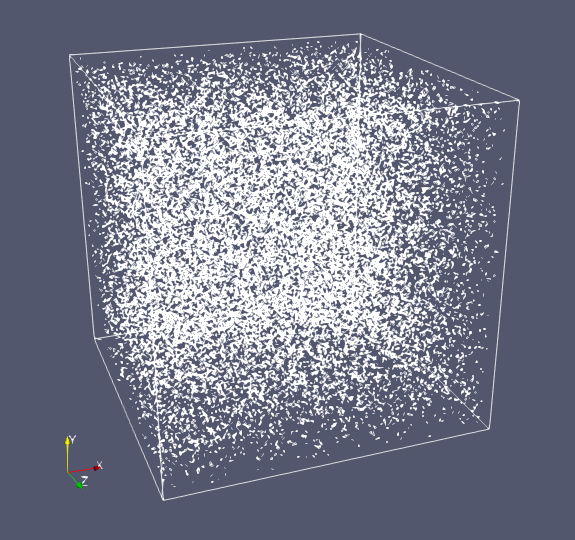
\includegraphics[width=\linewidth]{img/testcase-bench-mesh-1E5}
		\caption{$10^5$ Segments de taille $\unit{50}{\angstrom}$}
		\label{fig:testcase-bench-mesh-1E5}
	\end{subfigure}
	\begin{subfigure}{0.4\textwidth}
		\centering
		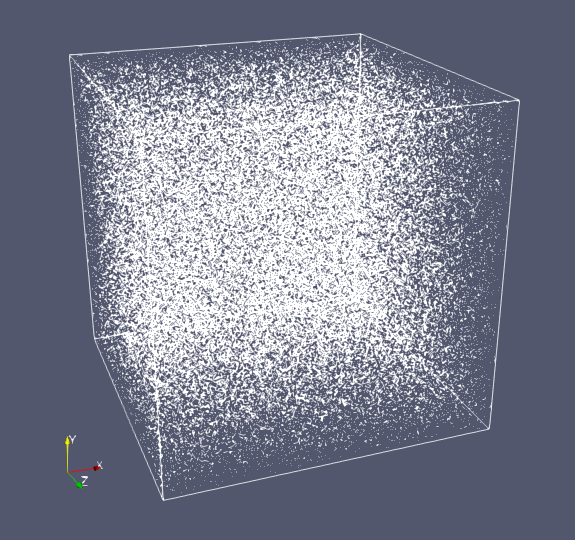
\includegraphics[width=\linewidth]{img/testcase-bench-mesh-1E6}
		\caption{$10^6$ Segments de taille $\unit{5}{\angstrom}$}
		\label{fig:testcase-bench-mesh-1E6}
	\end{subfigure}	
	\caption{Données générées pour tester la performance des parcours de la structure de données. Taille de domaine :\unit{1}{\micro\meter}; densité : $\unit{5\cdot 10^{14}}{\meter\per\meter\cubed}$ }
	\label{fig:testcase-bench-mesh}
\end{figure}

Pour le parcours témoin 'Stream', des tableaux de vecteurs à 3 dimensions de taille $S$ sont générés.

\subsubsection{Opérations effectuées pour chaque objet}

Pour chaque élément contenu dans la structure de données, on effectue un certain nombre d'opérations en fonction de l'intensité arithmétique $I$ demandée. La fonction exécutée pour chaque objet est décrite dans l'algorithme \ref{algo:function-bench-mesh}. 

\begin{algorithm}[H]
	\SetAlgoLined
	\LinesNumbered
	\SetAlgoNoEnd	
	\DontPrintSemicolon
	\SetKwInput{KwParams}{Paramètres}
	\KwParams{$I$ : L'intensité arithmétique}
	\KwData{$v_1$, $v_2$ et $v_3$ : des champs vectoriels de la structure de données.}
	
	$v_1 \leftarrow 0$\;
	\For{ $i$ dans $[1,I]$ }
	{
		$v_1 \leftarrow v_1 + (0.1 \cdot i )\cdot v_2 + (0.15 \cdot i) \cdot v_3$\;
	}
	
	\caption{Fonction exécutée pour chaque objet}
\end{algorithm}

La boucle for est en réalité implémentée en utilisant les templates afin que le compilateur puisse appliquer toutes les optimisations possibles. les $(0.1 \cdot i)$ et $(0.15 \cdot i)$ sont donc des constantes flottantes connues à la compilation différentes pour chaque multiplication. Cela permet de s'assurer que le compilateur ne factorise pas les multiplications, et effectue bien le nombre d'opérations flottantes attendu.

$v_1$, $v_2$ et $v_3$ sont des vecteurs en 3 dimensions en double précision. Pour chaque objet, 9 flottants doubles précisions (8 octets) sont chargés ou écrits. Le nombre d'octets écrits ou chargés au cours du parcours est:
\begin{equation}
	M(I,S) = 72 \cdot S
\end{equation}

Pour chaque objet, et pour chaque tour de boucle, on effectue 2 additions et 2 multiplications. Le nombre d'opérations flottantes au cours d'un parcours est le suivant:
\begin{equation}
	Flops(I,S) = 4 \cdot I \cdot S
\end{equation}

L'intensité en Flops/Octets en fonction de $I$ est :
\begin{equation}
	Intensite(I) = \frac{1}{18} \cdot I
\end{equation}

Selon les parcours considérés, les champs choisis pour $v_1$, $v_2$ et $v_3$ varient. 

\begin{table}
	\begin{tabulary}{1.0\textwidth}{r||c|C|C}
		\textbf{Parcours} & $\bm{v_1}$ & $\bm{v_2}$ & $\bm{v_3}$\\
		\hline
		\hline
		Référence & Tableau 1 & Tableau 2 & Tableau 3 \\
		\hline
		Nœuds seuls & Nouvelle position & Ancienne position & Vitesse\\
		\hline
		Segments avec Nœuds & Force sur le segment & Force nodale nœud 1 & Force nodale nœud 2\\
		\hline
		Nœuds avec Segments & Force nodale & Force sur le $1^{er}$ segment connecté & Force sur le  $2^{eme}$ segment connecté\\
	\end{tabulary}
	\caption{ Champs choisis pour le benchmark des parcours }
\end{table}

\subsubsection{Méthode de mesure du temps d'exécution}

La mesure du temps d'exécution des parcours de la structure de données se fait en utilisant des timers à grain fin à l'intérieur du code. La mesure retenue est le temps mesuré le plus court entre le début et la fin du parcours sur un échantillon de 100 parcours identiques. Cette mesure semble fiable, car elle est comparable à la moyenne des temps mesurés sur les 99 itérations, en omettant la $1^{ere}$ mesure (effets de cache). Cette méthode de mesure est inspirée du benchmark Stream \footnote{benchmark stream}.

\subsection{Performance des parcours en mémoire partagée.}

Cette section s'intéresse à la performance de la structure de données en mémoire partagée avec OpenMP. Nous proposons une méthode pour vérifier que la structure de données utilise correctement le matériel dans un contexte multithreadé sur un seul nœud de calcul. 

\subsubsection{Roofline Model et Machine de test}

Le roofline model est une représentation graphique de la performance d'une application. Il permet de comparer la puissance théorique du matériel à la vitesse d'exécution de l'application\footnote{ref roofline}. La courbe tracée représente la performance en Flops\per\second en fonction de l'intensité arithmétique en Flops\per Octet. Le graphique se décompose en deux parties:
\begin{itemize}
	\item La performance maximale du matériel. Elle peut être mesurée ou déduite des spécifications constructeur.
	\item Les mesures de performances de l'application.
\end{itemize}

\paragraph{Performances de la machine de test}

La machine utilisée pour effectuer les mesures est le cluster de la Maison de la Simulation : Poincare\footnote{ref poincare}. La topologie d'un noeud de la machine est donnée par la figure \ref{fig:lstopo_poincare}.

\begin{figure}
	\centering
	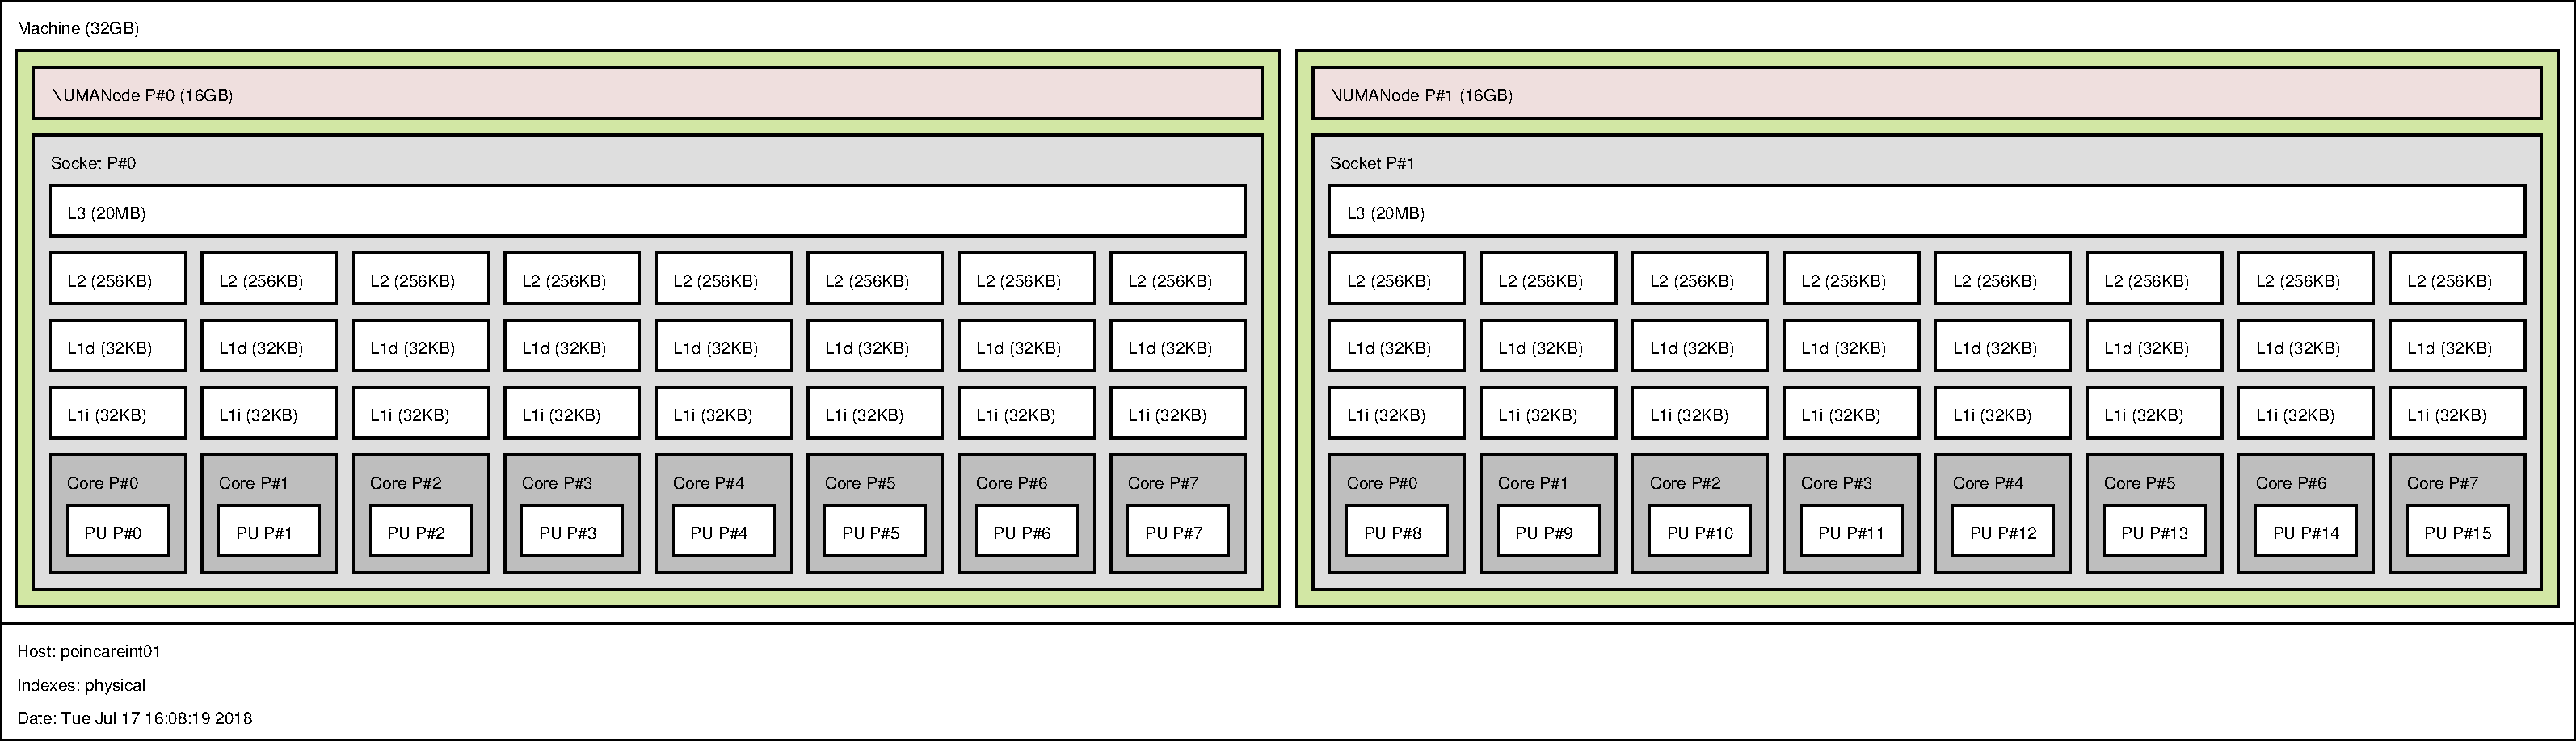
\includegraphics[width=\textwidth]{img/lstopo_poincare}
	\caption{Topologie d'un nœud de la machine Poincare}
	\label{fig:lstopo_poincare}
\end{figure}

La performance maximale d'un nœud de la machine Poincare est résumée dans les roofline models de la figure \ref{fig:roofline_poincare}. 

\begin{figure}
	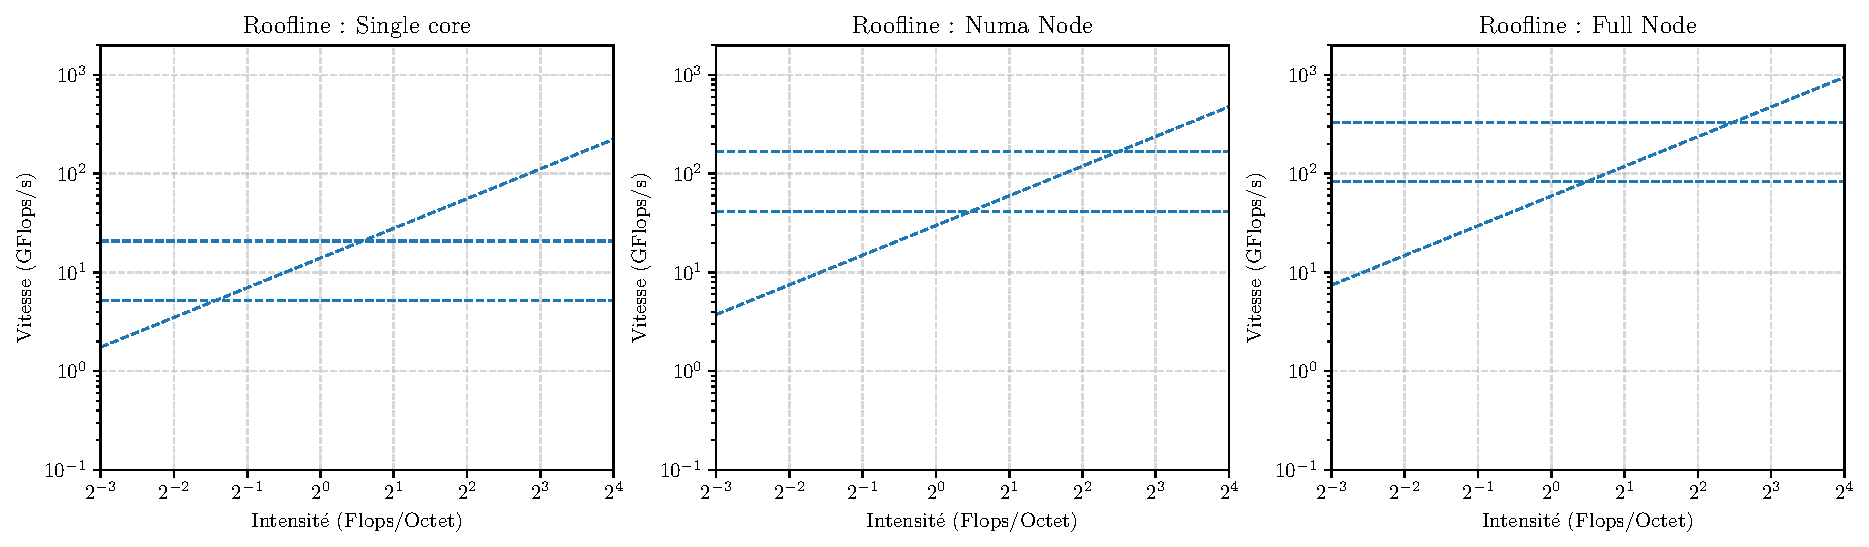
\includegraphics[width=\textwidth]{img/bench_mesh_roofline_limits}
	\caption{Performances de référence de la machine Poincare (Roofline)}
	\label{fig:roofline_poincare}
\end{figure}

Les 3 figures représentent les performances maximales de la machine avec différents nombre de threads.

La bande passante maximale (partie linéaire) à été mesurée en utilisant le benchmark Stream, et la performance crête (plateau) a été déduite des spécifications constructeur du processeur:
\begin{align}
	P_{AVX2} &=& \unit{2.6}{\giga\hertz} \times \unit{2}{ALUs} \times \unit{4}{double\per inst} &=& \unit{20.8}{GFlops\per\second\per coeur}\\
	P_{scalaire} &=& \unit{2.6}{\giga\hertz} \times \unit{2}{ALUs} \times \unit{1}{double\per inst} &=& \unit{5.2}{GFlops\per\second\per coeur}
\end{align}
Le tableau \ref{tab:perf_poincare} résume les performances maximales de la machine.

\begin{table}
	\begin{tabulary}{1.0\textwidth}{R||c|c|c}
		 & 1 coeur & 1 NUMA & Noeud complet\\
		\hline
		\hline
		Bande Passante ( \giga O\per\second ) & 14.0 & 29.9 & 59.5 \\
		Performance crête scalaire (\giga Flops\per\second) & 5.2 & 41.6 & 83.2 \\
		Performance crête AVX2 (\giga Flops\per\second)  & 20.8 & 166.4 & 332.8 \\
	\end{tabulary}
	\caption{ Performances maximales de la machine. }
	\label{tab:perf_poincare}
\end{table}

Une autre manière des présenter ces résultats pour les faible intensités arithmétiques est de tracer la courbe de la bande passante mesurée en fonction de l'intensité arithmétique. La figure \ref{fig:bench_mesh_bande_passante} affiche les bandes passantes maximales du matériel sur 3 graphiques, en fonction du nombre de threads utilisés.

\begin{figure}
    \centering
    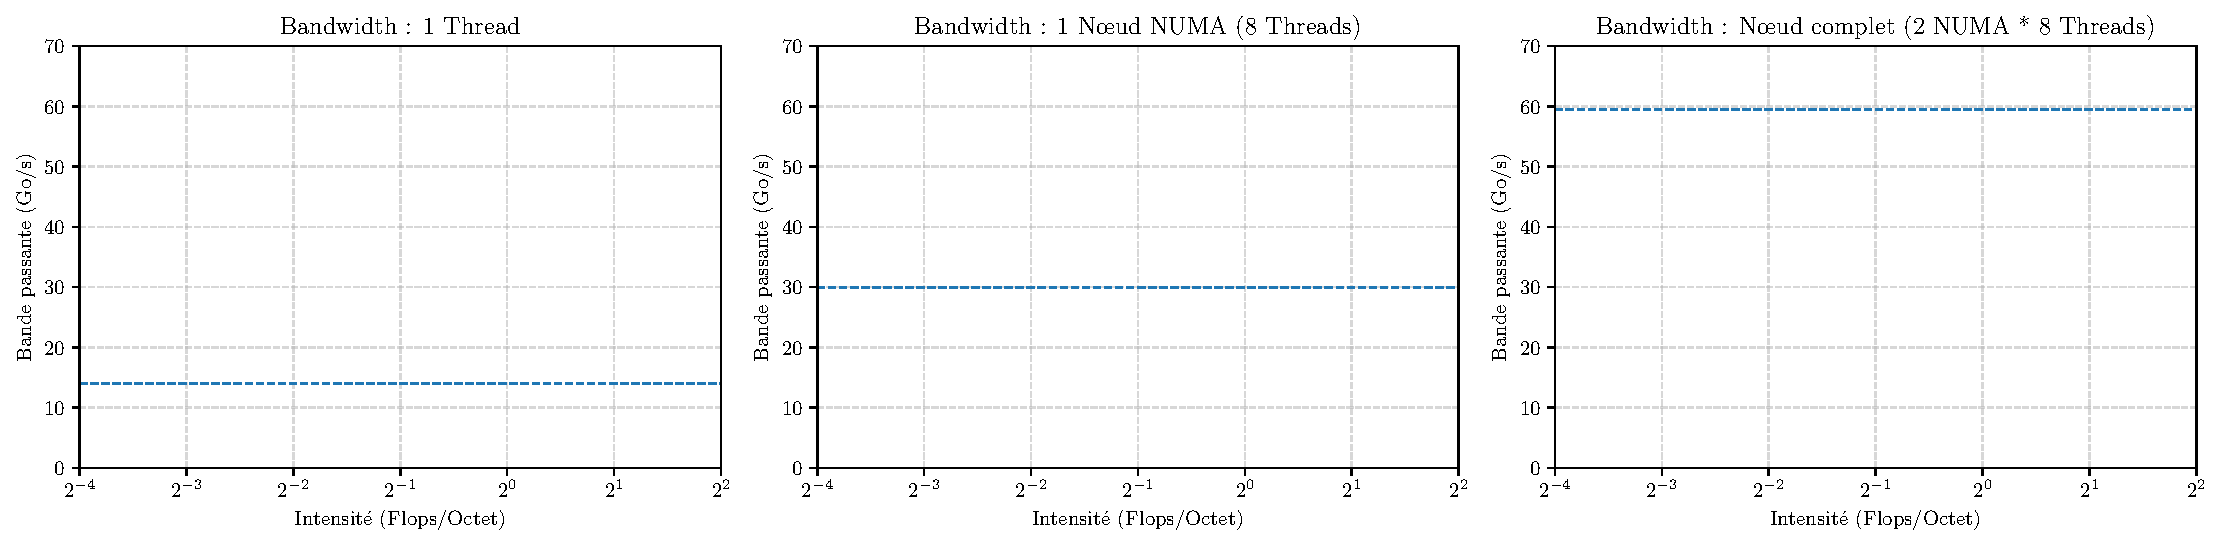
\includegraphics[width=\textwidth]{img/bench_mesh_bande_passante}
    \caption{Performances de référence de la machine Poincare (Bande passante)}
    \label{fig:bench_mesh_bande_passante}
\end{figure}

\paragraph{Placement des algorithmes sur le roofline}

Il est possible de calculer l'intensité arithmétique pour les algorithmes implémentés au sein d'optidis afin de les placer sur le Roofline model. Nous avons choisis d'étudier plusieurs algorithmes qui ont des propriétés différentes:
\begin{itemize}
    \item Le déplacement des nœuds du réseau de dislocation, qui présente une faible intensité arithmétique;
    \item Le calcul de l'incrément de déformation, qui possède une intensité arithmétique moyenne;
\end{itemize}

La figure \ref{fig:movenodes} est un extrait de code de la fonction chargée de déplacer les nœuds à leur nouvelle position en fonction de la vitesse calculée au préalable. En plus de calculer la nouvelle position, la fonction enregistre la position précédente. Cette fonction est prise comme exemple afin d'expliquer comment est calculée l'intensité arithmétique théorique d'une boucle. 

\begin{figure}
    \centering
    \begin{subfigure}[b]{0.47\textwidth}
        \centering
        \begin{minted}{c++}
    double dt;
    [...]
    MeshHelper::foreach_node( mesh, 
    [dt](Mesh::NodeInfo_ref& n)
    {
        n.x_old() = n.x();
        n.y_old() = n.y();
        n.z_old() = n.z();
        n.x() += dt*n.vx();
        n.y() += dt*n.vy();
        n.z() += dt*n.vz();
    });
    [...]
        \end{minted}
    \end{subfigure}
    \caption{Code : déplacement des nœuds}
    \label{fig:movenodes}
\end{figure}

A chaque itération, des champs de la structure sont chargés ou écrits en mémoire:
\begin{itemize}
    \item Position \mintinline{c++}{{n.x(),n.y(),n.z()}} : lecture + écriture
    \item Vitesse \mintinline{c++}{{n.vx(),n.vy(),n.vz()}} : lecture seule
    \item Ancienne vitesse \mintinline{c++}{{n.x_old(),n.y_old(),n.z_old()}} : écriture seule
\end{itemize}
Pour un total de 12 flottants double précision lus ou écrits. Le volume d'opérations mémoire par itération est donc:
\begin{equation}
    M = 12 \cdot \text{sizeof}(\texttt{double}) = \unit{96}{Octets}
\end{equation}

On compte 3 additions et 3 multiplications:
\begin{equation}
F = F_{add} + F_{mul} = \unit{6}{Flops}
\end{equation}

On en déduit l'intensité arithmétique :
On compte 3 additions et 3 multiplications:
\begin{equation}
I = F/M = \unit{\frac{1}{16}}{Flops/Octet} = \unit{0.0625}{Flops/Octet}
\end{equation}

De la même manière, on calcule l'intensité arithmétique pour les autres boucles, et on obtient le tableau \ref{tab:intensite_optidis}.

\begin{table}
    \centering
    \begin{tabulary}{1.0\textwidth}{r||c|C|C}
        \textbf{Algorithme} & \textbf{F (Flops)}&  \textbf{M (Octets)} & \textbf{I (Flops/Octet)} \\
        \hline
        \hline
        Déplacement des nœuds & $6$ & $96$ & $0.0625$ \\
        \hline
        Incrément de déformation & $72$ & $96$ & $0.75$ \\
    \end{tabulary}
    \caption{ Calcul des intensités arithmétiques de différents algorithmes au sein d'optidis. }
    \label{tab:intensite_optidis}
\end{table}

Il est alors possible de les placer sur un roofline, comme le montre la figure \ref{fig:roofline_algos}. Cette figure représente les limites théoriques du matériel sur un noeud NUMA de poincare sous forme de roofline model.

\begin{figure}
    \centering
    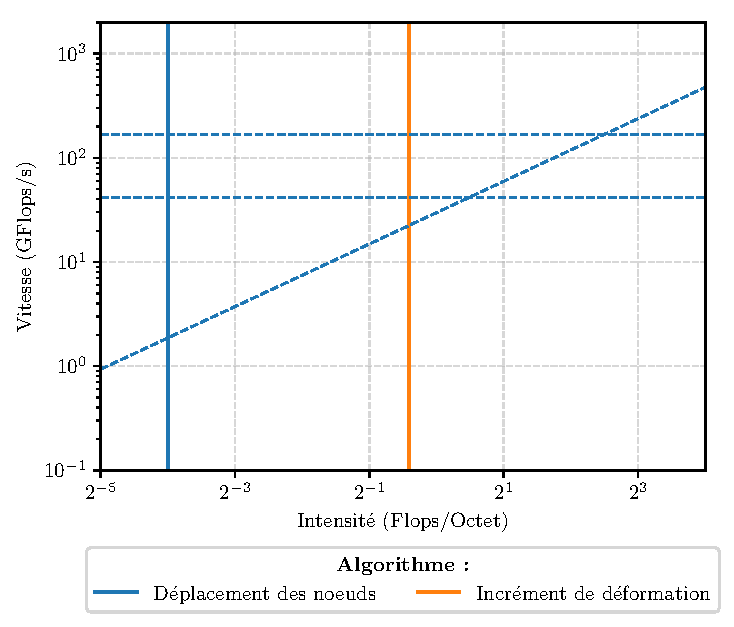
\includegraphics[width=.4\textwidth]{img/bench_mesh_roofline_algos.pdf}
    \caption{Roofline model pour un noeud NUMA de Poincare avec les intensités arithmétiques des algorithmes pris en exemple. }
    \label{fig:roofline_algos}
\end{figure}



\subsubsection{Comportement général}

Toutes les mesures effectuées sont consultables dans l'annexe \ref{annexe:bench_mesh}.

Les graphiques de la figure \ref{fig:bench_mesh_comportement_general} donnent un aperçu de la performance des parcours de la structure de données dans le cas qui représente le mieux son utilisation dans optidis. 

\begin{figure}
    \centering
    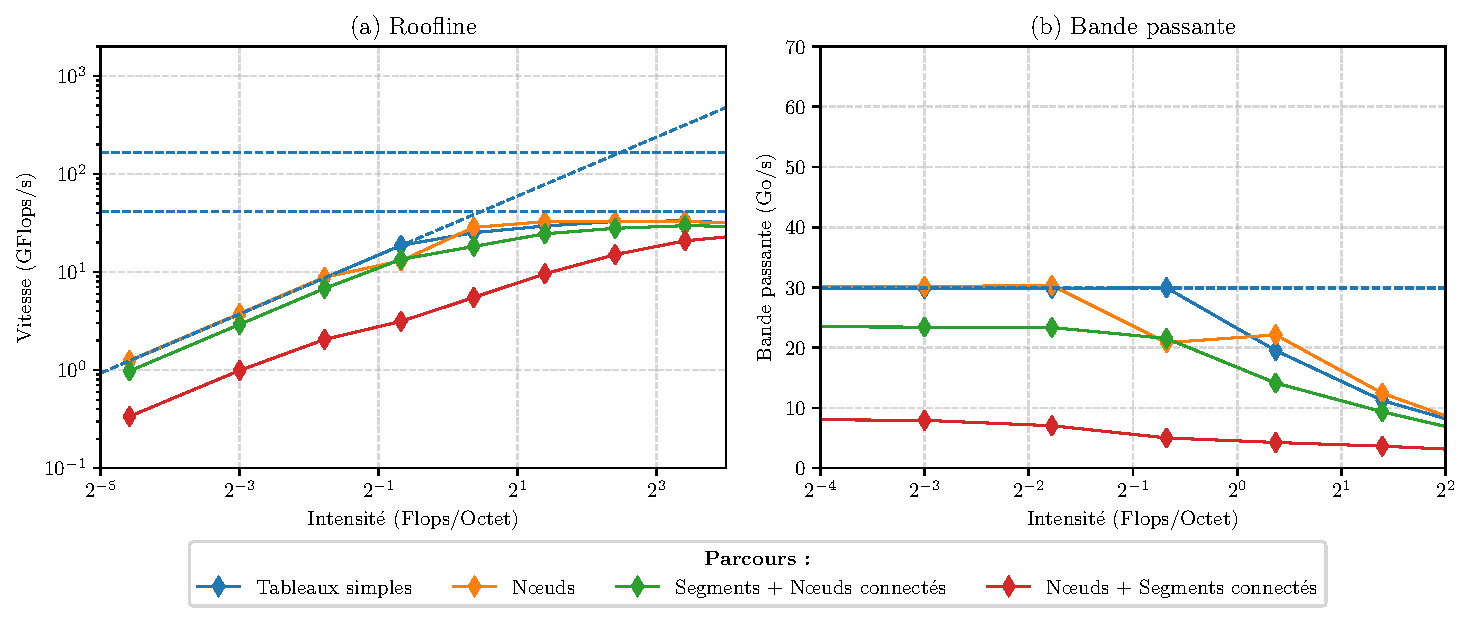
\includegraphics[width=0.8\textwidth]{img/bench_mesh_omp.pdf}
    \caption{Performance des parcours de la structure de données pour un volume de données dépassant la capacité du cache L3 ($10^6$ éléments) sur un nœud NUMA (8 threads)}
    \label{fig:bench_mesh_comportement_general}
\end{figure}

On remarque que dans ces conditions, les parcours de la structure de données utilisent efficacement les capacités de la machine. Les différents parcours ont des performances variables en accord avec la complexité des schémas d'accès aux données. Dans l'ordre, du parcours le plus performant au moins performant :
\begin{itemize}
    \item Le parcours de référence utilisant des tableaux simples montre des performances comparables aux performances maximales de la machine sans vectorisation ni effets de cache
    \item Le parcours des nœuds seuls montre une performance comparable au parcours de référence, ce qui montre que la couche d'abstraction ajoutée par la structure de données ne crée pas d'overhead.
    \item Le parcours des Segments avec nœuds connectés est un peu moins performant que les deux parcours précédent car le schéma d'accès aux données est plus complexe : il faut effectuer une indirection supplémentaire pour accéder aux segments connectés. On observe une bande passante utile inférieure de 20\% à la bande passante du parcours de référence.
    \item Le parcours des Nœuds avec Segments connectés possède des performances bien moindres car les nombre de segments connectés à un nœud est variable, ce qui empêche un certain nombre d'optimisations par le compilateur \footnote{ex : unrolling de la boucle sur les segments (c.f. intel advisor)}.
\end{itemize}

\subsubsection{Effets de la taille des données}

Le nombre d'objets contenu dans la structure de données joue un rôle important dans la performance des parcours, surtout pour les faibles intensités arithmétiques. La figure \ref{fig:bench_mesh_effet_taille} compare les performances des parcours sous forme de roofline et de graphe de bande passante pour $10^5$ et $10^6$ éléments sur un nœud NUMA.

\begin{figure}
    \centering
    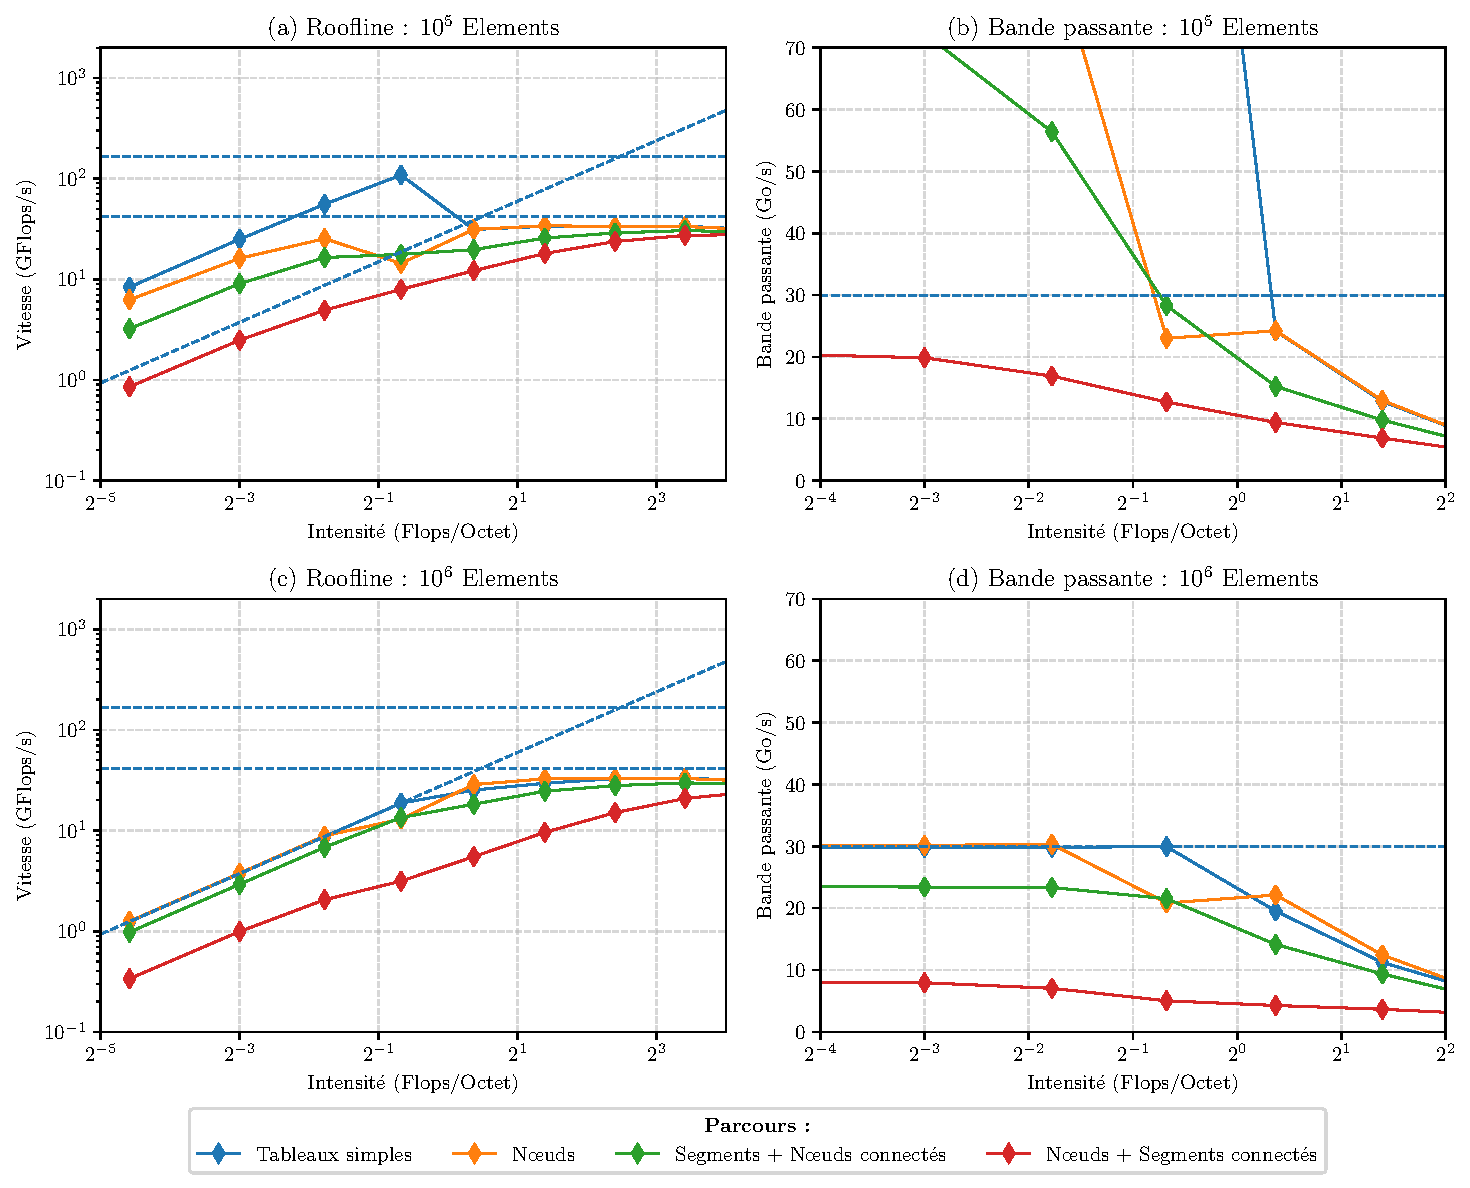
\includegraphics[width=.8\textwidth]{img/bench_mesh_omp_effet_taille.pdf}
    \caption{Impact du nombre d'objets contenus dans la structure sur un noeud NUMA (8 threads)}
    \label{fig:bench_mesh_effet_taille}
\end{figure}

Dans optidis les données sont souvent évincées du cache par des données extérieures (Octree FMM) et différents champs de la structure sont utilisées. Les algorithmes implémentés dans optidis ne peuvent donc pas bénéficier d'effets de cache sur la structure de données entre les itérations. On retiendra donc les mesures pour des données ne tenant pas en cache afin de mesurer la performance des parcours.

Il est possible d'améliorer la performance des algorithmes au sein d'optidis à l'intérieur d'une itération en utilisant du blocking pour les opérations à faible intensité arithmétique afin de bénéficier des effets de cache. 

\subsubsection{Effets du nombre de threads}

La figure \ref{fig:bench_mesh_effet_threads} compare la performance des parcours d'une structure de données contenant $10^6$ objets en fonction du nombre de threads utilisés.

\begin{figure}
    \centering
    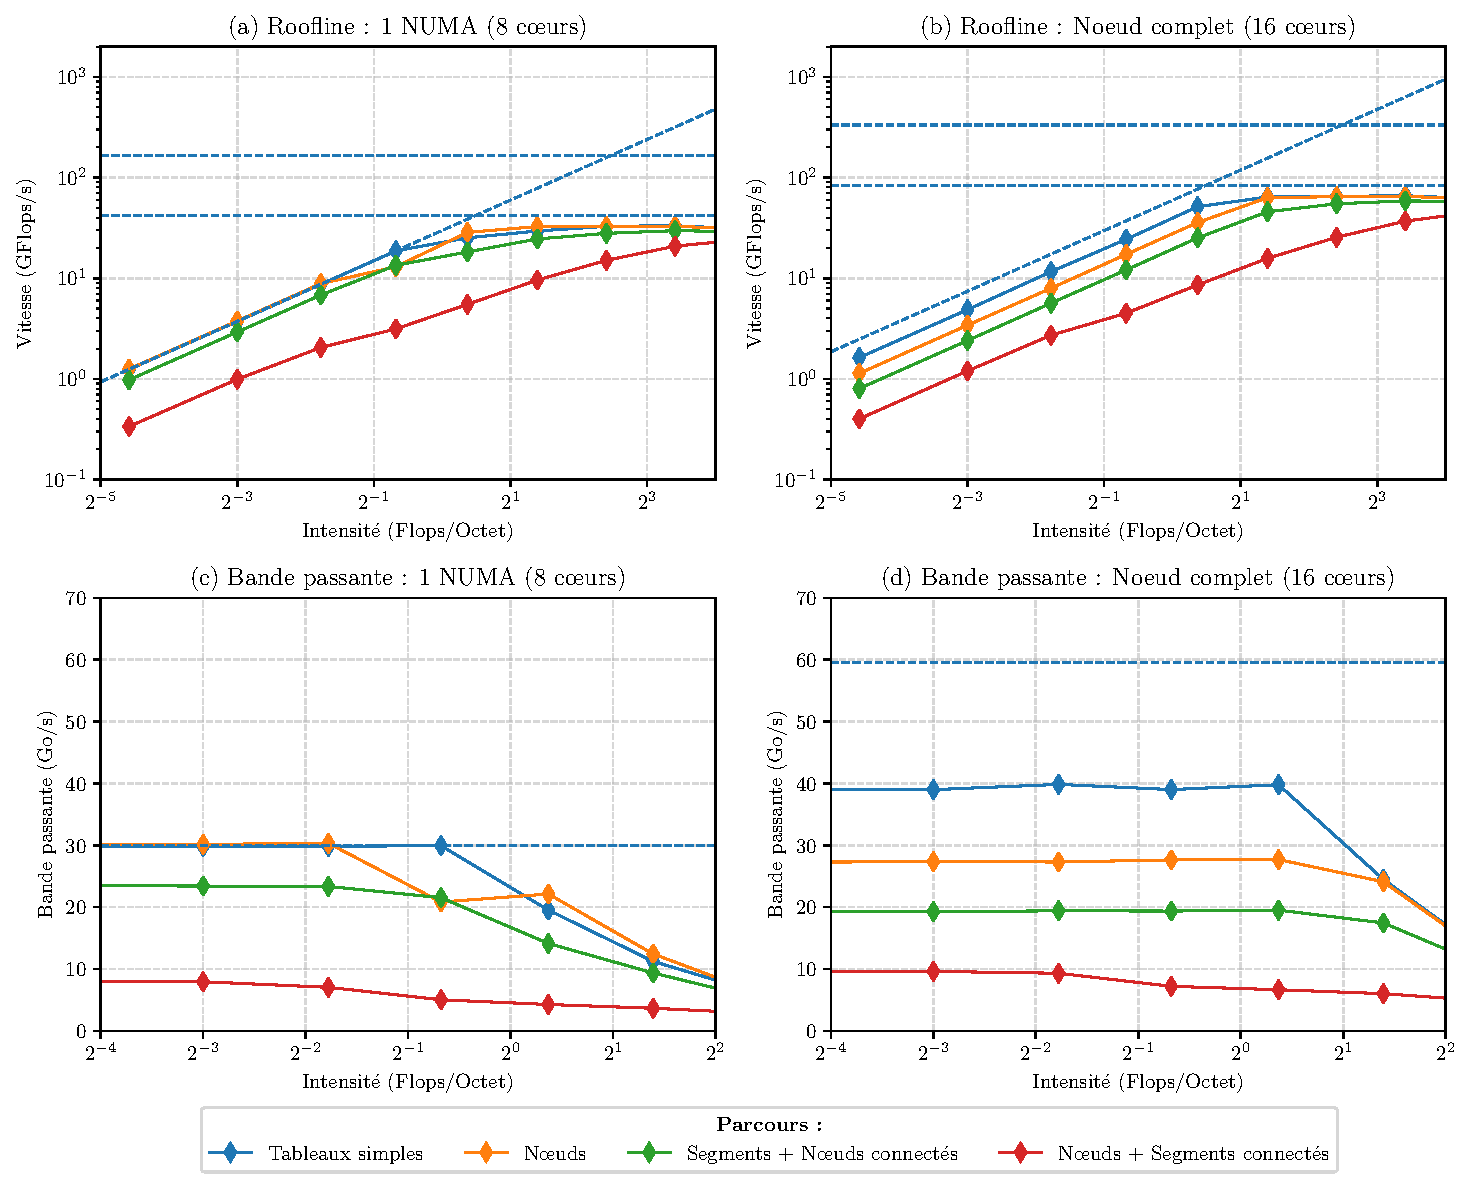
\includegraphics[width=0.8\textwidth]{img/bench_mesh_omp_effet_threads.pdf}
    \caption{Impact du nombre de threads sur la performance de la structure de données pour $10^6$ objets}
    \label{fig:bench_mesh_effet_threads}
\end{figure}

L'ajout d'un second noeud NUMA pour le parcours devrait permettre de doubler la bande passante utile, comme on peut l'observer dans une certaine mesure pour le parcours de référence. Cependant, pour les faibles intensités arithmétiques, les parcours de la structure de données ne bénéficient pas de l'ajout d'un 2eme nœud NUMA. Les mesures de bande passantes donnent des chiffres comparables que l'on utilise 1 ou 2 nœuds NUMA pour effectuer le parcours de la structure. En parallélisme hybride, il vaudra mieux utiliser un noeud NUMA par processus MPI.

\subsection{Environnement MPI}

Dans cette section, nous verrons comment se comporte la structure de données lorsque les objets sont distribués sur plusieurs processus MPI. Les graphiques proposés représentent le temps ou l'efficacité en fonction du nombre de processus MPI. Pour chacun des graphiques présentés, certaines grandeurs sont fixées.
\begin{itemize}
    \item Les mesures sont toujours effectuées sur un nœud NUMA (8 treads), car c'est le nombre de threads le plus adapté à la structure selon la section \ref{sec:bench_mesh_impact_threads}
    \item Le nombre d'éléments pourra être $10^5$ ou $10^6$ et sera indiqué sur chaque graphe
    \item L'intensité arithmétique pourra 
\end{itemize}

\subsection{Performance des opérations topologiques}